\documentclass[a4paper,12pt]{article}
\usepackage[T1]{fontenc}
\usepackage{tikz}
\usetikzlibrary {calc,graphs,graphs.standard,patterns.meta}
\usepackage[dvipsnames]{xcolor}
\usepackage{skak}
\usepackage{chessboard}
\usepackage{physics}
\tikzdeclarepattern{
name=mylines,
parameters={
\pgfkeysvalueof{/pgf/pattern keys/size},
\pgfkeysvalueof{/pgf/pattern keys/angle},
\pgfkeysvalueof{/pgf/pattern keys/line width},
},
bounding box={
(0,-0.5*\pgfkeysvalueof{/pgf/pattern keys/line width}) and
(\pgfkeysvalueof{/pgf/pattern keys/size},
0.5*\pgfkeysvalueof{/pgf/pattern keys/line width})},
tile size={(\pgfkeysvalueof{/pgf/pattern keys/size},
\pgfkeysvalueof{/pgf/pattern keys/size})},
tile transformation={rotate=\pgfkeysvalueof{/pgf/pattern keys/angle}},
defaults={
size/.initial=5pt,
angle/.initial=45,
line width/.initial=.4pt,
},
code={
\draw [line width=\pgfkeysvalueof{/pgf/pattern keys/line width}]
(0,0) -- (\pgfkeysvalueof{/pgf/pattern keys/size},0);
},
}

\begin{document}
\section{Recap}
Topology
Euler Characteristic

\section{Problems}

Several knights are situated on a 3 x 3 chessboard as shown in the Figure 1. Can they move, using the usual chess knight's move, to the position shown in Figure 2?

\setchessboard{
normalboard,
maxfield=c3,
setpieces={na1,nc1,Na3,Nc3},
showmover=false}
\chessboard

\setchessboard{
normalboard,
maxfield=c3,
setpieces={na1,Nc1,Na3,nc3},
showmover=false}
\chessboard

There are 9 computers connected with several cables to make a network. (Each cable connects a pair of machines.) Is it possible for each computer to be connected to exactly 3 others?



In Kottayam, there are 9 constituencies; some are connected by roads, and others are not. (A road connects a pair of constituencies with each other.) Is it possible that each of the constituencies is connected to exactly 3 other constituencies?



It is known that in a certain company, each employee has exactly 3 friends among the co-workers. Is it possible that this company has exactly 9 employees?

It is known that 3 edges meet at every vertex of a polyhedron. Is it possible for this polyhedron to have exactly 9 vertices?

\subsection{Graph Recap}
Vertices
Edges

Scenarios as graphs

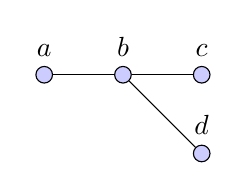
\begin{tikzpicture}
\graph [
    nodes={
        circle,
        draw,
        fill=blue!20,      % Fills the circle with a color
        minimum size=6pt,  % Reduces the radius/size of the circle
        inner sep=0pt      % Removes internal padding so it stays small
    },
    empty nodes            % Clears the default text from inside the circles
]
{ 
    a[label=above:$a$] -- 
    b[label=above:$b$] -- 
    {
        c[label=above:$c$], 
        d[label=above:$d$]
    } 
};
\end{tikzpicture}
vertices
edges

4 people, all friends with each other
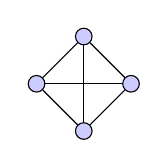
\begin{tikzpicture}
\graph [
    nodes={
        circle,
        draw,
        fill=blue!20,      % Fills the circle with a color
        minimum size=6pt,  % Reduces the radius/size of the circle
        inner sep=0pt      % Removes internal padding so it stays small
    },
    empty nodes            % Clears the default text from inside the circles
]{ subgraph K_n [--
, n=4, clockwise, radius=6mm] };
\end{tikzpicture}

4 computers, each connected to 2 others,
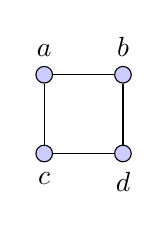
\begin{tikzpicture}
\graph [
    nodes={
        circle,
        draw,
        fill=blue!20,      % Fills the circle with a color
        minimum size=6pt,  % Reduces the radius/size of the circle
        inner sep=0pt      % Removes internal padding so it stays small
    },
    empty nodes,            % Clears the default text from inside the circles
    no placement
]
{ 
    a[label=above:$a$] -- { 
        b[at={(1,0)},label=above:$b$] -- {d[at={(1,-1)},label=below:$d$]}, 
        c[at={(0,-1)},label=below:$c$] -- d
    },
    % Connect the bottom row of nodes
    % b -- d
    
};
\end{tikzpicture}

% a[at={(0:0)}] -> b[] -> c[yshift=1cm];

a molecule of methane, $CH_4$, with 1 atom of carbon $(C)$ connected to 4 atoms of hydrogen $(H)$.

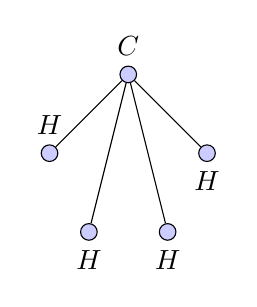
\begin{tikzpicture}
\graph [
    nodes={
        circle,
        draw,
        fill=blue!20,      % Fills the circle with a color
        minimum size=6pt,  % Reduces the radius/size of the circle
        inner sep=0pt      % Removes internal padding so it stays small
    },
    empty nodes,            % Clears the default text from inside the circles
    no placement
]
{ 
    a[at={(0,2)},label=above:$C$] -- { 
        b[at={(-1,1)},label=above:$H$], 
        c[at={(-1/2,0)},label=below:$H$],
        d[at={(1/2,0)},label=below:$H$], 
        e[at={(1,1)},label=below:$H$] 
    },    
};
\end{tikzpicture}

Can you model these problems as graphs?

\section{Problems to calculate the number of edges in a graph}

A couple invites 10 people to a house party. The hosts shake hands with everyone but each other. The guests shake hands with everyone else in the party. How many handshakes took place?

IRTC has 9 computers. They want to link them into a network so that every computer would be connected with exactly 4 computers by network cables.
(a) How many cables will they need? Can you draw such a configuration?
(b) They decided to connect every computer with exactly 5 other computers. Is this a possible configuration?


During a chess tournament some people played 5 games and some people played 6. Can you show that the number of people who played 5 games is even?

Degree of a vertex: The number of edges that start at a given vertex is called the degree of a vertex.


A vertex can have degree 0.

a graph that has every vertex connected to every other is called complete.

For any graph the number of vertices with an odd degree must be even. (Go back to the computer network problem)

calculate the total number of edge ends 

1. the total number of edge ends is equal to the sum of the degrees of the vertices

2. the total number of edge ends is equal to twice the total number of edges in the graph = even

$\implies$ sum of the degrees of the vertices is even
$\implies$ even number of odd degree vertices

\section{Sperner's Lemma}

\begin{tikzpicture}
    \coordinate (A) at (0,0);
    \coordinate (B) at (6,0);
    \coordinate (C) at (3,4);
    \coordinate (ab1) at ($ (A)!.25!(B) $);
    \coordinate (ab2) at ($ (A)!.55!(B) $);
    \coordinate (ab3) at ($ (A)!.85!(B) $);
    \filldraw [SkyBlue] (A) circle [radius=2pt];
    \filldraw [Orange] (B) circle [radius=2pt];
    \filldraw [darkgray] (C) circle [radius=2pt];

    \draw (A) -- (B) -- (C) -- cycle;
    \filldraw [SkyBlue] (ab1) circle [radius=2pt];
    \filldraw [Orange] (ab2) circle [radius=2pt];
    \filldraw [SkyBlue] (ab3) circle [radius=2pt];

    \coordinate (ac1) at ($ (A)!.25!(C) $);
    \coordinate (ac2) at ($ (A)!.55!(C) $);
    \coordinate (ac3) at ($ (A)!.85!(C) $);

    \filldraw [SkyBlue] (ac1) circle [radius=2pt];
    \filldraw [darkgray] (ac2) circle [radius=2pt];
    \filldraw [darkgray] (ac3) circle [radius=2pt];

    \coordinate (bc1) at ($ (B)!.25!(C) $);
    \coordinate (bc2) at ($ (B)!.55!(C) $);
    \coordinate (bc3) at ($ (B)!.85!(C) $);

    \filldraw [Orange] (bc1) circle [radius=2pt];
    \filldraw [darkgray] (bc2) circle [radius=2pt];
    \filldraw [darkgray] (bc3) circle [radius=2pt];

    \coordinate (r1) at ($ (ac1)!.25!(bc1) $);
    \draw (r1) circle [radius=2pt];
    \filldraw [Orange] (r1) circle [radius=2pt];

    \coordinate (r2) at ($ (ac1)!.45!(bc1) $);
    \draw (r2) circle [radius=2pt];
    \filldraw [SkyBlue] (r2) circle [radius=2pt];

    \coordinate (r3) at ($ (ac1)!.8!(bc1) $);
    \draw (r3) circle [radius=2pt];
    \filldraw [darkgray] (r3) circle [radius=2pt];

    \coordinate (r4) at ($ (ac2)!rnd!(bc2) $);
    \draw (r4) circle [radius=2pt];
    \filldraw [Orange] (r4) circle [radius=2pt];

    \draw (ac1) -- (bc1);
    \draw (ac2) -- (bc2);
    \draw (ac3) -- (bc3);
    \draw (ac1) -- (ab1) -- (r1) -- (ab2) -- (r2) -- (ab3) -- (r3) -- (B);
    \draw (ac2) -- (r1) -- (r4) -- (r2) -- (bc2) -- (r3);
    \draw (ac3) -- (r4) -- (bc3);

    \draw[pattern={mylines[size= 5pt,line width=.8pt,angle=40]},
pattern color=red] (ab3) -- (r3) -- (B) -- cycle;
    \draw[pattern={mylines[size= 5pt,line width=.8pt,angle=40]},
pattern color=red] (ac1) -- (r1) -- (ac2) -- cycle;

    \draw[pattern={mylines[size= 5pt,line width=.8pt,angle=40]},
pattern color=red] (r2) -- (r4) -- (bc2) -- cycle;
\end{tikzpicture}

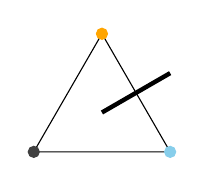
\begin{tikzpicture}
\draw (-30:1) -- (90:1) -- (210:1) --cycle;
\draw[ultra thick] (0:0) -- (30:1);
\filldraw [SkyBlue] (-30:1) circle [radius=2pt];
\filldraw [Orange] (90:1) circle [radius=2pt];
\filldraw [darkgray] (210:1) circle [radius=2pt];
\end{tikzpicture}

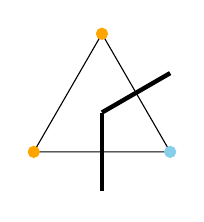
\begin{tikzpicture}
\draw (-30:1) -- (90:1) -- (210:1) --cycle;
\draw[ultra thick] (0:0) -- (-90:1);
\draw[ultra thick] (0:0) -- (30:1);
% \draw[ultra thick] (0:0) -- (150:1);
\filldraw [SkyBlue] (-30:1) circle [radius=2pt];
\filldraw [Orange] (90:1) circle [radius=2pt];
\filldraw [Orange] (210:1) circle [radius=2pt];
\end{tikzpicture}

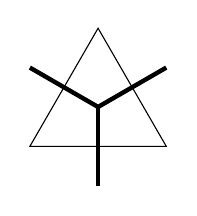
\begin{tikzpicture}
\draw (-30:1) -- (90:1) -- (210:1) --cycle;
\draw[ultra thick] (0:0) -- (-90:1);
\draw[ultra thick] (0:0) -- (30:1);
\draw[ultra thick] (0:0) -- (150:1);
\end{tikzpicture}

See the skeleton as a graph.
What are its properties?
Take the centers of the small triangles as the vertices.
Notice degree of the vertices, possibilities as 0, 1, 2

Look at the edges of the boundaries, orange blue boundary, how many edges exiting the boundary?
How many external vertices can we have?
Odd number external vertices.

Sum of the degrees of all vertices should be an even = 2 times number of edges

sum of external contribution = odd

sum of degrees of internal vertices = odd

number of internal with degree 1 = odd number

What changes can we make to the boundary conditions?

Preserve external vertices = odd (any pair of colors)

Triangulation : Divide into triangles

Can you write an algorithm to find the multiculored triangles?

Can you force the arrangement to have exactly 1 multicolored triangle?

What is the largest number of multicolored triangle you can obtain and what configuration will realise this?
\section{Components}

Two vertices are connected if there is a path that links them. A path is a sequence of connected edges.

A component is a set of connected vertices. If two vertices are not connected, they belong to different components.
\subsection{Problem}
Hypothetical scenario: In Thodupuzha (a taluk in Idukki) there is only one mode of transportation: KSRTC Bus. Twenty-five buses serve the Thodupuzha town. A single bus line serves Kaliyar, and every other panchayat is served by exactly 10 bus lines. Show that it is possible to travel by bus from the Thodupuzha town to Kaliyar (perhaps with several transfers).

Hint: Proof by Contradiction

25 + 10n = odd
1 + 10m = odd

Graphs with odd numbers of odd vertices are impossible. Is the opposite equally true?

The 8 heads of state of SAARC got together for a conference. According to a reporter, each of the heads of Afghanistan, Bangladesh, and Bhutan shook hands with 6 heads of state each, each of the heads of India, Maldives, and Nepal with 4, and each of the heads of Pakistan, and Sri Lanka with 1. Is the reporter correct?

Solve these problems ins Groups:

Can you draw a graph that has 5 vertices, in which the degrees of these vertices are 4, 4, 4, 2, and 2? Either draw such a graph or explain why it is impossible.


Problem 2.
(a) Can you draw a graph that has 8 vertices, each of degree 3?
(b) Can you draw a graph that has 21 vertices, each of degree 3?
(c) Can you draw a graph that has 20 edges, with all of its vertices having a degree of 3?
For each part, either draw such a graph or explain why such a graph is impossible.

15 students registered for the summer maths camp. It is known that every participant is acquainted with at least 7 more students from his school who registered for the same camp. Show that all the children are, in fact, from the same school.

There are 12 towns on the Island of Knights and Liars; roads connect some of them. Charlie claims that a different number of roads start in each town. Prove that Charlie is a Liar.

\section{Transport problem}
A farmer has to take a tiger, a goat, and some melons across a river. Their boat has enough room for themself plus either the tiger, the goat, or the melons. If they take the melons with them, the tiger will eat the goat. If they takes the tiger across, the goat will eat the melons. Only when the farmer is present are the goat and the melons safe from their enemies. All the same, the farmer successfully carries the tiger, the goat, and the melons across the river. How?

(F,T,G,M) ()
(T,M) (F,G)
(F,T,M) (G)
(M) (F,T,G)
(F,G,M) (T)
(G) (F,M,T)
(F,G) (M,T)
() (F,G,M,T)
\section{Edge Coloring}

In a group of 6 students, every pair of students are either friends or enemies. Prove that it is possible to choose 3 of these students so that they are either all friends or all enemies.


\section{More Problems}
% \setchessboard[]
% \newchessgame
% \chessboard


\end{document}